\documentclass[a4paper,10pt]{article}
\usepackage[utf8x]{inputenc}
\usepackage{graphicx}

%opening
\title{Informe tarea algoritmos probabilísticos}
\author{María Andrea Cruz Blandón \and Edgar Andrés Moncada Taborda \and Luis Felipe Vargas Rojas}

\begin{document}

\maketitle

\section{N-Reinas - Las Vegas}

En un experimento de 8-Reinas realizado 1000 veces se obtuvo el siguiente resultado:
\begin{itemize}
 \item Promedio de probabilidad de éxito, el cual se obtuvo a partir de las probabilidades parciales de cada uno de los 1000 intentos es: $0.3077625$. A continuación se muestras las gráficas 
relacionadas con las probabilidades obtenidas, en una observamos como fueron las probabilidades en cada uno de los intentos y en el orden en que sucedieron, y en la otra veremos los intentos
ordenados por el valor de la probabilidad, en ésta podemos observar que el algoritmo tienen inclusos momentos en que en el primer intento obtiene éxito.

\begin{figure}
 \centering
 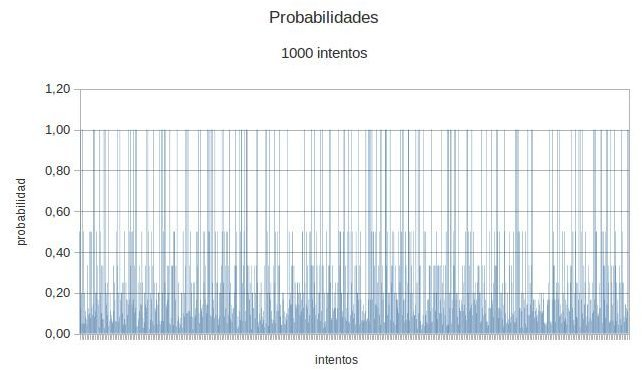
\includegraphics[scale=0.5]{promedios.jpg}
 \caption{Probabilidades de cada uno de los 1000 intentos}
 \label{fig:promedios}
\end{figure}

\begin{figure}
 \centering
 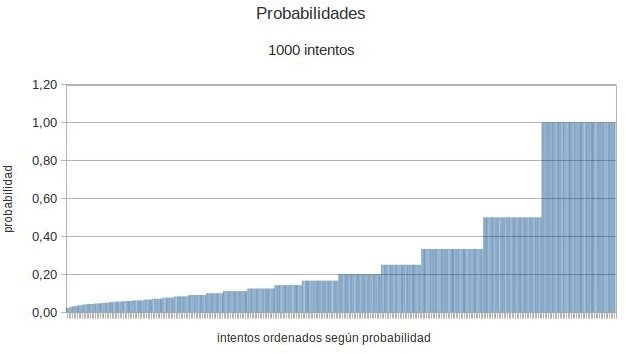
\includegraphics[scale=0.5]{probabilidadOrdenadas.jpg}
 \caption{1000 intentos ordenados por las probabilidades obtenidas}
 \label{fig:proOrden}
\end{figure}

\item Para analizar el tiempo esperado para el éxito, se contabilizó cuantas reinas se habían colocado en cada fracaso antes de que se diera dicho éxito. una vez tenemos este número procedemos a sacar
el promedio de los 1000 intentos para así obtener en número de reinas cuantas son necesarias para llegar al éxito. De este análisis se obtuvieron dos resultados, uno que en promedio son necesarios $6,577$ 
fracasos antes de encontrar el éxito aunque se alcanzaron numero de fracaso de hasta $39$. El segundo resultado tiene que ver con la cantidad de reinas que en promedio se insertaron en los fracasos
antes de dar con el éxito, aquí encontramos que en promedio (promedio de los promedios de los 1000 intentos) se necesitan $5,166$ reinas para encontrar el éxito.En la gráfica relacionada a la cantidad de reinas
promedio que se insertaron antes del éxito se observa cierta uniformidad. También debemos resaltar que 6 reinas insertadas conforma el $75\%$ de las reinas que se necesitan insertar y si este número
lo multiplicamos por el promedio de fracasos obtenemos que en promedio se están insertando $33,977$ reinas antes de encontrar el éxito.

\begin{figure}
 \centering
 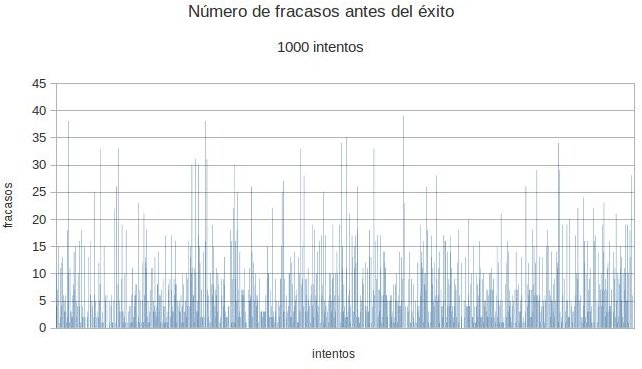
\includegraphics[scale=0.5]{fracasos.jpg}
 % fracasos.jpg: 642x369 pixel, 72dpi, 22.65x13.02 cm, bb=0 0 642 369
 \caption{Fracasos obtenidos antes del éxito en cada uno de los 1000 intentos}
 \label{fig:fracasos}
\end{figure}


\begin{figure}
 \centering
 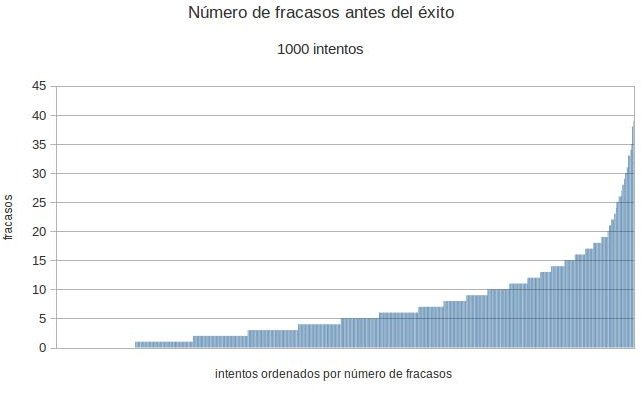
\includegraphics[scale=0.5]{fracasosOrden.jpg}
 % fracasosOrden.jpg: 642x393 pixel, 72dpi, 22.65x13.86 cm, bb=0 0 642 393
 \caption{Intentos ordeandos por numero de fracasos antes del éxito}
 \label{fig:fracasosOr}
\end{figure}


\begin{figure}
 \centering
 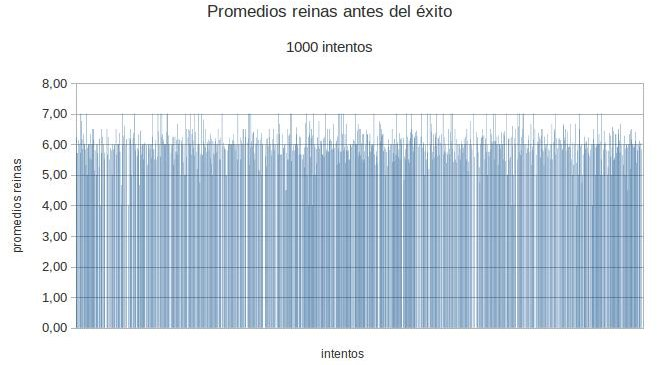
\includegraphics[scale=0.5]{reinaspromedio.jpg}
 % reinaspromedio.jpg: 657x365 pixel, 72dpi, 23.18x12.88 cm, bb=0 0 657 365
 \caption{Reinas promedio insertadas en cada fracaso antes de encontrar el éxito.}
 \label{fig:reinasprom}
\end{figure}

\item Para analizar el tiempo en que se demoraba en asignar posibles posiciones para luego elegir una aleatoriamente, se realizó el promedio por intento (fracaso-éxito), Así como se analizó
el número de reinas que se insertaron antes del éxito. Con lo anterior obtuvimos un promedio de $3,136$ posibles de los promedios de los 1000 intentos. En la gráfica podemos observar como este
promedio se mantiene con cierta uniformidad alrededor de 3 posibles.

\begin{figure}
 \centering
 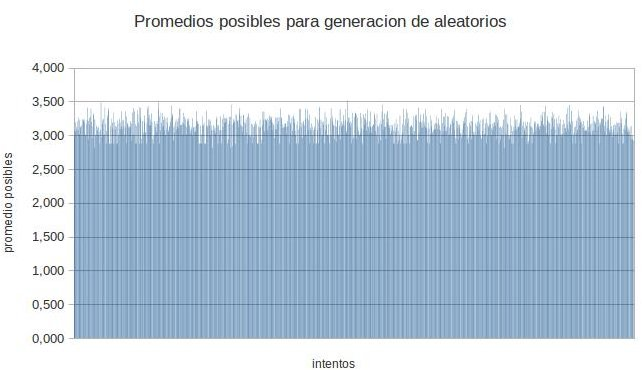
\includegraphics[scale=0.5]{promediosposibles.jpg}
 % promediosposibles.jpg: 816x1056 pixel, 72dpi, 28.79x37.25 cm, bb=0 0 816 1056
 \caption{Posibles antes de calcluar la posición aleatoria}
 \label{fig:posibles}
\end{figure}

\item Para determinar los intervalos de confianza usamos $\alpha = 0.05$ por lo que obtenemos $z=\pm1.96$ Despejamos de la formula para halla el intervalo.\\

\begin{eqnarray}
-1.96 \leq& \frac{X -  \mu}{\frac{ \sigma}{\sqrt{1000}}} &\leq 1.96\\ 
X - 1.96 \cdot{\frac{ \sigma}{\sqrt{1000}}} \leq&  \mu &\leq X + 1.96 \cdot{\frac{ \sigma}{\sqrt{1000}}}
\end{eqnarray}
A continuación los diferentes promedios y sus intervalos de confianza. \\

Probabilidad de obtener éxito: \\

Desviación estándar: 0,304\\
Promedio obtenido (X): 0.308\\
Intervalo: $0,289 \leq \mu \leq 0,327$\\

Promedio reinas insertadas en un intento:\\

Desviación estándar: 2,112\\
Promedio obtenido (X): 5,166\\
Intervalo: $5,035 \leq \mu \leq 5,297$\\

Promedio fracasos antes del éxito:\\

Desviación estándar: 6,734 \\
Promedio obtenido (X): 6,577 \\
Intervalo: $6,160 \leq \mu \leq 6,994$ \\

Promedio posibles posiciones (demora para poder asignar una posición aleatoria):\\

Desviación estándar: 0,136 \\
Promedio obtenido (X): 3,136\\
Intervalo: $ 3,128 \leq \mu \leq 3,144$ \\

\end{itemize}


Realizando el experimento con 10-Reinas:

\begin{itemize}
 \item Probabilidad de éxito obtenida: $0,180\%$
 \item Intervalo de confianza: \\
  Desviación estándar: 0,242 \\
  Promedio obtenido (X): 0,180\\
  Intervalo: $ 0,165 \leq \mu \leq 0,195$ \\
 \item Gráficos de probabilidades obtenidas en los 1000 intentos.

\begin{figure}
 \centering
 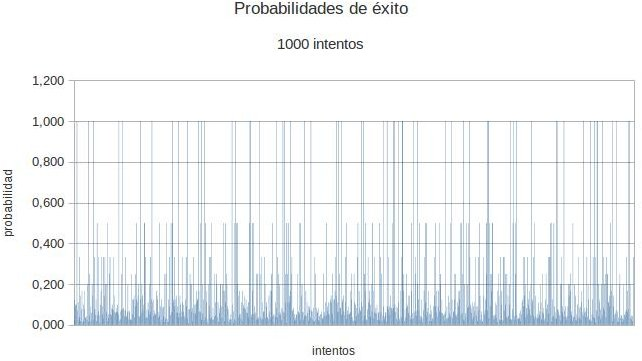
\includegraphics[scale=0.5]{probabilidad10.jpg}
 % probabilidad10.jpg: 642x361 pixel, 72dpi, 22.65x12.74 cm, bb=0 0 642 361
 \caption{Probabilidad de obtener éxito 10-Reinas}
 \label{fig:probabilidad10}
\end{figure}

\begin{figure}
 \centering
 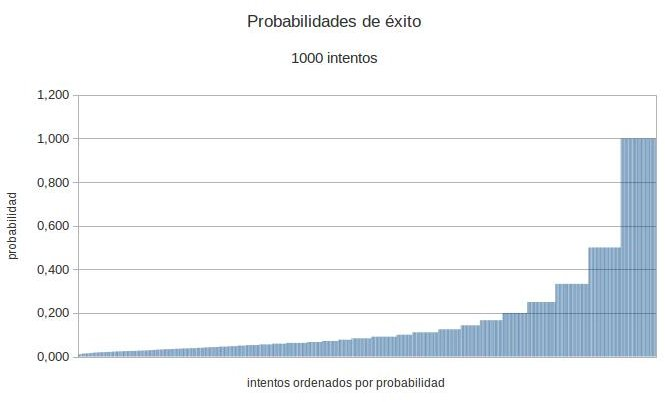
\includegraphics[scale=0.5]{probabilidadOrden10.jpg}
 % probabilidadOrden10.jpg: 665x402 pixel, 72dpi, 23.46x14.18 cm, bb=0 0 665 402
 \caption{Intentos ordenados por probabilidades obtenidas en cada intento. 10-Reinas}
 \label{fig:probaOrd10}
\end{figure}

\item Fracasos antes del éxito se obtuvo como promedio: $15,434$
\item Máximo número de fracasos obtenidos: $125$
\item Intervalo de confianza: \\
  Desviación estándar: 15,814 \\
  Promedio obtenido (X): 15,434\\
  Intervalo: $ 14,454  \leq \mu \leq 16,414$ \\

\item Gráficos de número de fracasos antes del éxito.

\begin{figure}
 \centering
 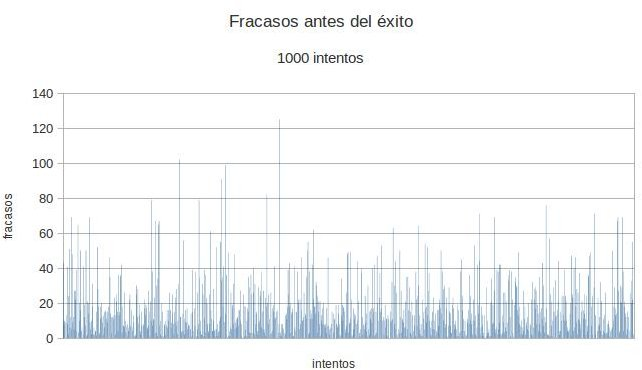
\includegraphics[scale=0.5]{fracasos10.jpg}
 % fracasos10.jpg: 642x370 pixel, 72dpi, 22.65x13.05 cm, bb=0 0 642 370
 \caption{Número de fracasos obtenidos en cada uno de los 1000 intentos antes de obtener el éxito. 10-Reinas}
 \label{fig:fracasos10}
\end{figure}

\begin{figure}
 \centering
 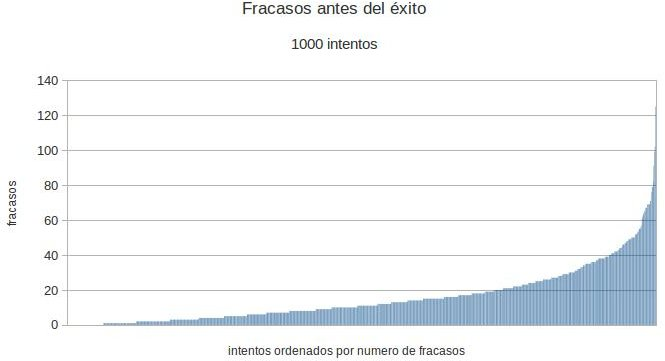
\includegraphics[scale=0.5]{fracasosOrd10.jpg}
 % fracasosOrd10.jpg: 665x361 pixel, 72dpi, 23.46x12.74 cm, bb=0 0 665 361
 \caption{Intentos ordenados por el número de fracasos obtenidos antes del éxito. 10-Reinas}
 \label{fig:fracasos10Ord}
\end{figure}

\item Número de reinas insertadas en cada intento (fracaso-éxito), se obtuvo en promedio: $7,753$
\item Intervalo de confianza:
  Desviación estándar: 0,739 \\
  Promedio obtenido (X): 7,753\\
  Intervalo: $ 7,707  \leq \mu \leq 7,799$ \\

\item Con el número de fracasos promedio y numero de reinas insertadas promedio obtenemos que en promedio se insertan por intento (hasta obtener éxito) $119,660$ reinas.
\item Gráfica que muestra comportamiento uniforme alrededor de 7 reinas insertadas en cada intento (fracaso-éxito)

\begin{figure}
 \centering
 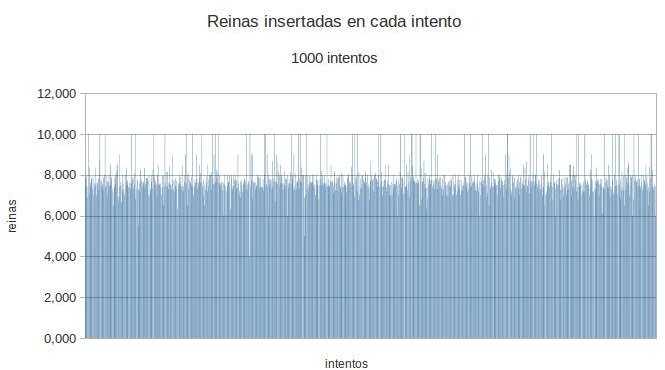
\includegraphics[scale=0.5]{reinas10.jpg}
 % reinas10.jpg: 816x1056 pixel, 72dpi, 28.79x37.25 cm, bb=0 0 816 1056
 \caption{Reinas promedio insertadas en cada intento. 10-Reinas}
 \label{fig:rinas10}
\end{figure}

\item Promedio de posibles lugares para generar la posición aleatoria, el obtenido fue de: $3,846$
\item Intervalo de confianza:
  Desviación estándar: 0,166 \\
  Promedio obtenido (X): 3,846\\
  Intervalo: $ 3,836 \leq \mu \leq 3,856$ \\

\item En la gráfica podemos observar cierta uniformidad respecto al número de espacios explorados en promedio para poder asignar una posición aleatoria a una reina. este número resulta
bastante cercano al encontrado en el experimento con 8-Reinas.

\begin{figure}
 \centering
 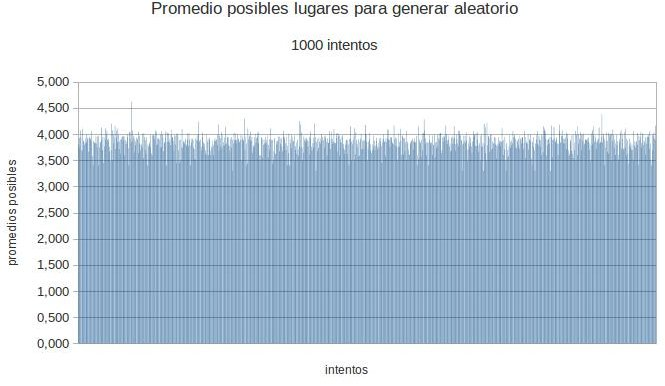
\includegraphics[scale=0.5]{posibles10.jpg}
 % posibles10.jpg: 665x386 pixel, 72dpi, 23.46x13.62 cm, bb=0 0 665 386
 \caption{Promedio posibles lugares para asignar una posición aleatoria a una reina. 10-Reinas}
 \label{fig:posibles10}
\end{figure}

\end{itemize}

Realizando el experimento con 15-Reinas:

\begin{itemize}
 \item Probabilidad de éxito obtenida: $0,130\%$
 \item Intervalo de confianza: \\
  Desviación estándar: 0,212 \\
  Promedio obtenido (X): 0,130\\
  Intervalo: $ 0,117 \leq \mu \leq 0,143$ \\
 \item Gráficos de probabilidades obtenidas en los 1000 intentos.

\begin{figure}
 \centering
 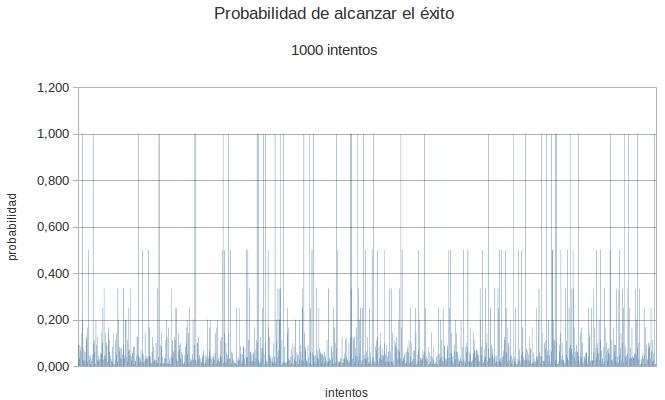
\includegraphics[scale=0.5]{probabilidad15.jpg}
 % probabilidad15.jpg: 665x400 pixel, 72dpi, 23.46x14.11 cm, bb=0 0 665 400
 \caption{Probablidades obtenidas en los 1000 intentos. 15-Reinas}
 \label{fig:prob15}
\end{figure}

\begin{figure}
 \centering
 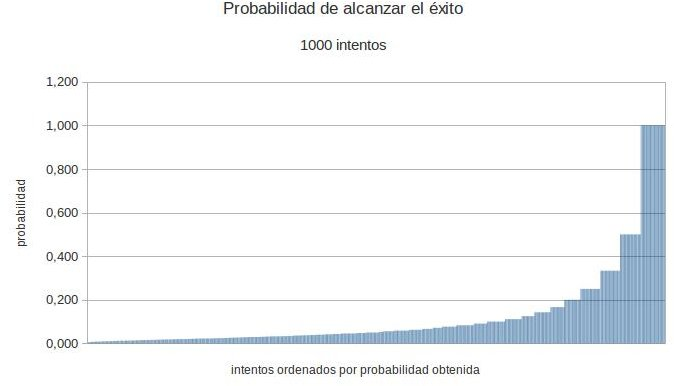
\includegraphics[scale=0.5]{./probabilidadOrden15.jpg}
 % probabilidadOrden15.jpg: 674x386 pixel, 72dpi, 23.78x13.62 cm, bb=0 0 674 386
 \caption{Intentos ordenados por probabilidad obtenidad. 15-Reinas}
 \label{fig:prob15Ord}
\end{figure}

\item Fracasos antes del éxito se obtuvo como promedio: $27,624$
\item Máximo número de fracasos obtenidos: $313$
\item Intervalo de confianza: \\
  Desviación estándar: 29,955 \\
  Promedio obtenido (X): 27,624\\
  Intervalo: $ 25,767  \leq \mu \leq 29,481$ \\

\item Gráficos de número de fracasos antes del éxito.

\begin{figure}
 \centering
 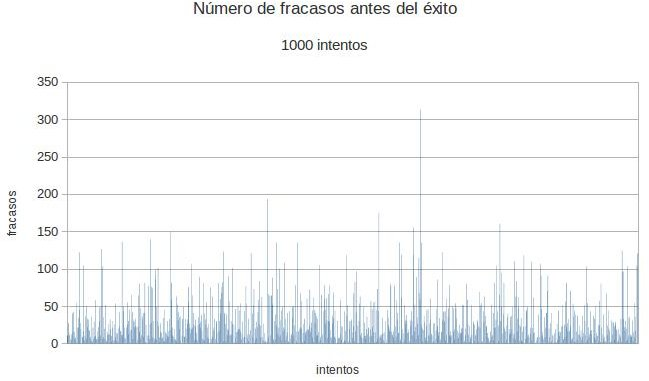
\includegraphics[scale=0.5]{fracasos15.jpg}
 % fracasos10.jpg: 642x370 pixel, 72dpi, 22.65x13.05 cm, bb=0 0 642 370
 \caption{Número de fracasos obtenidos en cada uno de los 1000 intentos antes de obtener el éxito. 15-Reinas}
 \label{fig:fracasos15}
\end{figure}

\begin{figure}
 \centering
 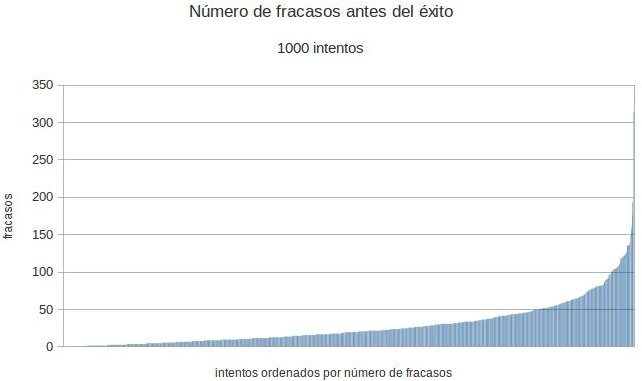
\includegraphics[scale=0.5]{fracasosOrd15.jpg}
 % fracasosOrd10.jpg: 665x361 pixel, 72dpi, 23.46x12.74 cm, bb=0 0 665 361
 \caption{Intentos ordenados por el número de fracasos obtenidos antes del éxito. 15-Reinas}
 \label{fig:fracasos15Ord}
\end{figure}

\item Número de reinas insertadas en cada intento (fracaso-éxito), se obtuvo en promedio: $11,814$
\item Intervalo de confianza:
  Desviación estándar: 0,846 \\
  Promedio obtenido (X): 11,814\\
  Intervalo: $ 11,762  \leq \mu \leq 11,866$ \\

\item Con el número de fracasos promedio y numero de reinas insertadas promedio obtenemos que en promedio se insertan por intento (hasta obtener éxito) $326,350$ reinas.
\item Gráfica que muestra comportamiento uniforme alrededor de 11 reinas insertadas en cada intento (fracaso-éxito)

\begin{figure}
 \centering
 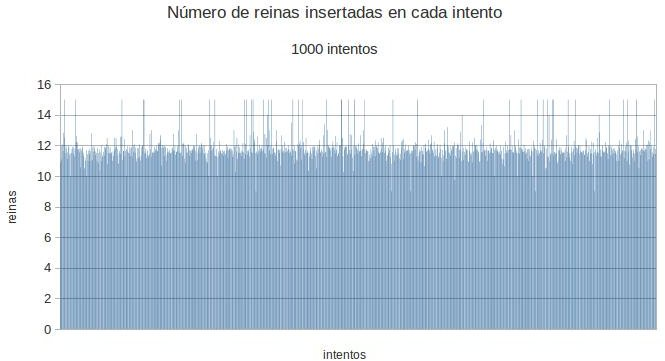
\includegraphics[scale=0.5]{reinas15.jpg}
 % reinas10.jpg: 816x1056 pixel, 72dpi, 28.79x37.25 cm, bb=0 0 816 1056
 \caption{Reinas promedio insertadas en cada intento. 15-Reinas}
 \label{fig:rinas10}
\end{figure}

\item Promedio de posibles lugares para generar la posición aleatoria, el obtenido fue de: $5,564$
\item Intervalo de confianza:
  Desviación estándar: 0,226 \\
  Promedio obtenido (X): 5,564\\
  Intervalo: $ 5,550 \leq \mu \leq 5,578$ \\

\item En la gráfica podemos observar cierta uniformidad respecto al número de espacios explorados en promedio para poder asignar una posición aleatoria a una reina.

\begin{figure}
 \centering
 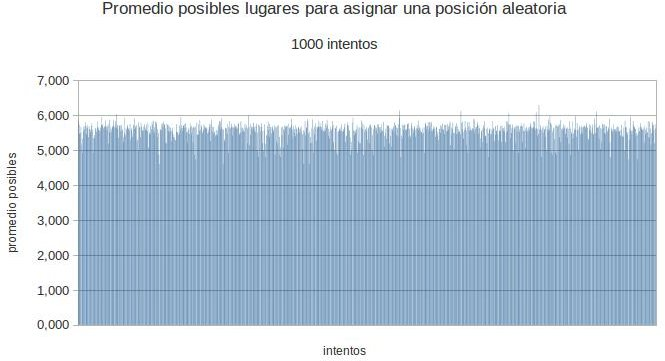
\includegraphics[scale=0.5]{posibles15.jpg}
 % posibles10.jpg: 665x386 pixel, 72dpi, 23.46x13.62 cm, bb=0 0 665 386
 \caption{Promedio posibles lugares para asignar una posición aleatoria a una reina. 15-Reinas}
 \label{fig:posibles10}
\end{figure}

\end{itemize}


\textbf{Conclusiones}\\

\begin{itemize}
 \item Realizando el experimento con diferente números de reinas, se puede observar como la probabilidad de alcanzar el éxito se ve fuertemente afectada por el número de reinas. Es una
relación inversamente proporcional, entre mas reinas se tiene mas baja es la probabilidad de éxito del algoritmo.
\item Un comportamiento que prevaleció en los 3 experimentos fue el correspondiente a el número de reinas insertadas en un intento, sea este un fracaso o un éxito. Se obtuvo que cerca del
del $70\%$ de las reinas se insertaban antes de obtener el éxito, osea con el $70\%$ de las reinas insertabas se caía en un fracaso.
\item Tanto el número de reinas insertadas en un intento como el número de posibles lugares explorados tienen un comportamiento uniforme en los 3 experimentos.
\item Este algoritmo presenta fuertes dificultades con el tamaño de la entrada respecto a encontrar una solución óptima sin embargo para entradas pequeñas como 8-Reinas, el algoritmo funciona
bastante bien, respecto a eficiencia.
\end{itemize}






\end{document}
